\documentclass[11pt, addpoints, answers]{exam}

\usepackage{amsmath, amssymb}
\usepackage{xcolor}
\usepackage{enumerate}
\usepackage{graphicx}
\usepackage{tabularx}
\usepackage{algorithm}
\usepackage{algpseudocode}
\usepackage{tikz}
\usepackage{tikz-qtree}
\usepackage{subfigure}

\newcommand{\red}[1]{\textcolor{red}{#1}}
\newcommand{\blue}[1]{\textcolor{blue}{#1}}

% For inserting code snippets.
\usepackage{listings}
\lstset{
    columns = fixed,
    basewidth = {0.5em},
    breaklines = true,
    backgroundcolor = \color{white},
    keywordstyle = \color[RGB]{40, 40, 255},
    numberstyle = \footnotesize\color{darkgray},
    commentstyle = \ttfamily\color{violet},
    basicstyle = \ttfamily,
    stringstyle = \ttfamily\color[RGB]{128, 0, 0},
    showstringspaces = false,
    language = {[11]C++},
    escapechar = \@
}
\lstnewenvironment{cpp}[1][]{\lstset{language = {[11]C++}, #1}}{}

\renewcommand{\baselinestretch}{1.15}
\setlength{\parskip}{1.25\baselineskip}

\usepackage{tikz}
\usepackage{tikz-qtree}
\tikzset{every tree node/.style={minimum width=2em,draw,circle},
    blank/.style={draw=none},
    edge from parent/.style=
    {draw,edge from parent path={(\tikzparentnode) -- (\tikzchildnode)}},
    level distance=1.2cm}



% headers, footers, titles
\newcommand{\CourseName}{CS101 Algorithms and Data Structures}
\newcommand{\HomeworkNO}{9}
\newcommand{\DueDate}{December 4, 2024}

\pagestyle{headandfoot}
\runningheadrule
\runningheader{CS101 Fall24}{Homework \HomeworkNO}{Due on: \DueDate}
\runningfooter{}{\thepage}{}

\title{
    \vspace{25pt}
    \LARGE ShanghaiTech University \\
    \bigskip
    \textbf{\CourseName} \\
    \textbf{Fall 2024}   \\
    \bigskip
    Homework \HomeworkNO
}
\author{}
\date{Due date: \DueDate, at 23:59}

% formats of questions, choices, points, etc.
\qformat{\bf\thequestion. (\totalpoints\ points) \thequestiontitle\hfill}
\pointname{'}
\CorrectChoiceEmphasis{\bf\color{blue}}
\SolutionEmphasis{\color{blue}}

% We frequently use this font.
\newcommand{\ttt}{\texttt}
\newcommand{\bluett}[1]{\textcolor{blue}{\ttt{#1}}}

\begin{document}

\maketitle

\vspace{50pt}

\begin{enumerate}
    \item Please write your solutions in English.
    \item Submit your solutions to Gradescope.
    \item Set your FULL name to your Chinese name and your STUDENT ID correctly in Gradescope account settings.
    \item If you want to submit a handwritten version, scan it clearly. \ttt{CamScanner} is recommended.
    \item We recommend you to write in \LaTeX.
    \item When submitting, match your solutions to the problems correctly.
    \item No late submission will be accepted.
    \item Violations to any of the above may result in zero points.
\end{enumerate}
\newpage

\begin{questions}

\titledquestion{Multiple Choices}

Each question has \textbf{one or more} correct answer(s). Select all the correct answer(s). For each question, you will get 0 points if you select one or more wrong answers, but you will get 1 point if you select a non-empty subset of the correct answers.

Write your answers in the following table.

%%%%%%%%%%%%%%%%%%%%%%%%%%%%%%%%%%%%%%%%%%%%%%%%%%%%%%%%%%%%%%%%%%%%%%%%%%%
% Note: The `LaTeX' way to answer a multiple-choice question is to replace `\choice'
% with `\CorrectChoice', as what you did in the first question. However, there are still
% many students who would like to handwrite their homework. To make TA's work easier,
% you have to fill in your selected choices in the table below, no matter whether you use 
% LaTeX or not.
%%%%%%%%%%%%%%%%%%%%%%%%%%%%%%%%%%%%%%%%%%%%%%%%%%%%%%%%%%%%%%%%%%%%%%%%%%%

\begin{table}[htbp]
	\centering
	\begin{tabular}{|p{2cm}|p{2cm}|p{2cm}|p{2cm}|p{2cm}|}
		\hline 
		(a) & (b) & (c) & (d)  \\
		\hline
  		%%%%%%%%%%%%%%%%%%%%%%%%%%%%%%%%%%%%%%%%%%%%%%%%%%%%%%%%%%
		% YOUR ANSWER HERE.
		   &  &  &  \\
            %%%%%%%%%%%%%%%%%%%%%%%%%%%%%%%%%%%%%%%%%%%%%%%%%%%%%%%%%%
		\hline
	\end{tabular} 
\end{table}

\begin{parts}


\part[2] Which of the following statements about topological sort is/are true?
\begin{choices}
    \choice A sub-graph of a DAG may not have a topological sorting.
    \choice Any directed tree has a topological sorting.
    \choice It's possible for a DAG to have multiple topological sortings.
    \choice Since we have to scan all vertices to find those with zero in-degree in each iteration, the run time of topological sort is $\Omega(|V|^2)$.
    
\end{choices}

\part[2] Which of the following statements about topological sort is/are true?

\begin{choices}

\choice For a connected graph, we can determine if it has a cycle in $\Theta(|E|)$ time.

\choice A critical path in a DAG is a path from the source to the sink with the maximum total weights.

\choice A DAG with all different weighted edges has one unique critical path.


\choice A DAG has at least one source and at least one sink.


\end{choices}

\part[2] Which of the following sequences is/are \textbf{Topological Sorting}(s) of the given DAG?
	\vspace{0.1in}
	\begin{center}
		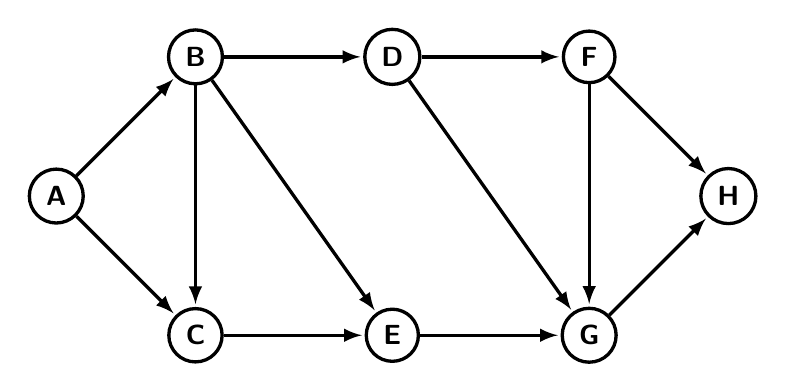
\begin{tikzpicture} [node distance = 2.5cm, very thick, main/.style = {draw, circle, font=\sffamily\bfseries}, edge/.style={->,> = latex, shorten > = 1pt}]
			\node[main] (B) {B};
                \node[main, below left of = B] (A) {A};
			\node[main, below  right of = A] (C) {C};
			\foreach \i\j in {B/D, D/F, C/E, E/G} {
					\node[main, circle, right of = \i] (\j) {\j};
				}
                \node[main, below right of = F] (H) {H};
			\draw[edge] (A) -- (B);
			\foreach \i\j in {B/C, A/C, B/D, D/F, C/E, E/G, B/E, D/G, F/H, G/H} {
					\draw[edge] (\i) -- (\j);
				}
			\draw[edge] (F) -- (G);
		\end{tikzpicture}
	\end{center}
	\begin{choices}
    	\choice 	    A B C E G D F H
		\choice 	A B C D E F G H
		\choice 	A B D C F E G H
		\choice 	    A B D E C F G H
	\end{choices}

\part[2]For the coin-changing problem, denote
    \begin{itemize}
        \item $C=(c_1, c_2,\cdots,c_k)$: the denominations of coins, where $1=c_1<c_2<\dots<c_k$;
        \item $X_n^*$: an optimal solution, i.e., a multi-set of coins which has the minimum number of coins to make change for $n$;
        \item $X_n$: the greedy solution, solved by
        \[
        X_n=\begin{cases}
        \{ \},&n=0\\
        \{c_t\}\cup X_{n-c_t},&n\ge 1, \text{where } c_t=\max\limits_{c_i\le n}c_i \text{ is the largest coin that can be used}
        \end{cases}
        \]
    \end{itemize}

For example, if $C=(1,2,3)$, then $X_4^*$ can be either $\{2,2\}$ or $\{3,1\}$, and $X_4=\{3,1\}$.

Which of the following statements is/are true?

    \begin{choices}
 
        \choice If $\forall i\in[3,n], c_i=c_{i-1}+c_{i-2}$, then $\forall n,|X_n^*|=|X_n|$.
        \choice $\exists C,\exists i$ with $2c_i>c_{i+1}$, such that $\forall n,|X_n^*|=|X_n|$.
        \choice If $\forall i, 2c_i\le c_{i+1}$, then $\forall n,|X_n^*|=|X_n|$.
        \choice If $\forall i\in[2,n], \dfrac{c_i}{c_{i-1}}$ is an integer, then $\forall n,|X_n^*|=|X_n|$.
 
    \end{choices}

\end{parts} 

\newpage



\titledquestion{Test Paper Arrangement Task}

Midterm week is finally over! Now the CS101 course staff is filing the test papers. Suppose there are $t$ test papers waited to be filed, and the course staff was assigned $n$ file cabinets with various capacities. Mark the capacity of the file cabinet as $c_i$ ($i = 1, 2, \cdots, n$). It's guaranteed that $\sum_{i = 1}^n c_i \geq t$.\\



\begin{parts}

\part[5] Given the number of test papers $t$ and the capacities of each of the $n$ cabinets $c_1, c_2, \cdots, c_n$, come up with a greedy algorithm that can file the papers in cabinets such that the least number of cabinets is used. You should give out the steps of your algorithm \textbf{(as efficient as possible)} and the time complexity (tight).

\newpage

\part[5] Prove the optimality of your algorithm using \textbf{Exchange Arguments} (any optimal solution can be iteratively exchanged to your greedy solution without making it worse). Answer the questions in step 4.5. to give your sufficient proof.\\
\textbf{Proof:}
\begin{enumerate}
    \item Assume $c_1>c_2>\cdots>c_n$ after sorted. Denote a solution $X=(x_1,x_2,\cdots,x_n)$ where we put $x_i$ test papers in the cabinet of capacity $c_i$. And the measurement $m(X)$ is counting how many cabinets have at least one test paper.
    \item Assume the optimal solution is $X^*$, and the greedy solution is $X$.
    \item Consider the first point of discrepancy between $X^*$ and $X$ at index $i$ (i.e. $x^*_i\ne x_i$).
    \item How to perform changes to make $x^*_i=x_i$? You should ensure that such changes is always valid in all possible scenarios of $X^*$.
    \begin{solution}
    
        \vspace*{5cm}
    \end{solution}
    \item Why such changes doesn't make $X^*$ worse? You should consider all possible scenarios of $X^*$.
    \begin{solution}
    
        \vspace*{5cm}
    \end{solution}
    \item Continue Applying steps 3.4.5. until $X^*=X$. Finally we prove that $X$ is an equally optimal solution.
\end{enumerate}

\end{parts}
\newpage


\titledquestion{Topological Sorting}

Consider the unweighted directed graph $G$ below. 

\begin{figure}[H]
    \centering
    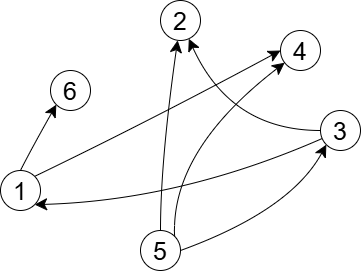
\includegraphics[width=0.5\linewidth]{fig/Topological_Sort.png}
    \label{fig:Topological_Sort}
\end{figure}

\begin{parts}

\part[5] 
How many topological sort results are there for the graph? State all possible results and show your calculated process.

\vspace{5cm}


\part[5] 
Construct an example of a single directed edge that, when added to $G$, would make it impossible to create a valid topological ordering of the graph. Then, determine the total number of such edges that could be added to $G$ and explain why each of these edges prevents a topological ordering.\\
(Ensure that this edge is not a self-loop and does not duplicate an existing edge in $G$.)

\vspace{5cm}

\end{parts}


\titledquestion{Greedy algorithm}
 
You are given a set of \( n \) cakes. Each cake \( i \) has:
\begin{itemize}
    \item A \textbf{satisfaction value} \( s_i\in\mathbb N^+ \), representing the enjoyment you get from eating the cake.
    \item An \textbf{expiration date} \( e_i\in\mathbb N^+ \), specifying the latest day (starting from day 1) the cake can be eaten. If not eaten by day \( e_i \), the cake is no longer valid.
\end{itemize}

You can eat at most \textbf{one cake per day}, starting from day 1, up to day $E=\max\limits_{i\in[1,n]} \{e_i\}$ i.e. the maximum expiration date of any cake. Your goal is to determine the best strategy to eat the cakes to \textbf{maximize the total satisfaction}, defined as the sum of the satisfaction values of the cakes you consume.

To illustrate, consider the following example of \( n = 9 \) cakes:

\[
\begin{array}{|c|c|c|c|c|c|c|c|c|c|c|}
    \hline
    i & \textbf{1} & \textbf{2} & \textbf{3} & \textbf{4} & \textbf{5} & \textbf{6} & \textbf{7} & \textbf{8} & \textbf{9} \\ \hline
    s_i & 10 & 20 & 10 & 15 & 14 & 40 & 18 & 5 & 20 \\ \hline
    e_i & 5 & 3 & 3 & 3 & 5 & 4 & 5 & 7 & 5 \\ \hline
\end{array}
\]

The maximum expiration date is \( m=7 \), so you need to decide which cake to eat on each day from day \( 1 \) to day \( 7 \). Note that:
\begin{itemize}
    \item You can only eat cake \( i \) on day \( j \) if \( j \leq e_i \), due to the expiration date constraint.
    \item You can leave some days without eating any cake if that results in a higher total satisfaction.
\end{itemize}

We represent a possible allocation as \( C=\{c_1, c_2, \dots, c_E\} \), where \(c_j\) is the index of the cake eaten on day \( j \), and ``-" indicates no cake is eaten on that day.

Here are three valid allocations for this example:
\begin{itemize}
    \item \( \{1, 2, 3, 5, 7, 8, -\} \), with a total satisfaction of \( 77 = 10 + 20 + 10 + 14 + 18 + 5 \).
    \item \( \{1, 2, 3, 6, 7, -, 8\} \), with a total satisfaction of \( 103 = 10 + 20 + 10 + 40 + 18 + 5 \).
    \item \( \{2, 4, 6, 7, 9, -, 8\} \), with a total satisfaction of \( 118 = 20 + 15 + 40 + 18 + 20 + 5 \).
\end{itemize}

For this instance, one of the optimal allocations is \( \{2, 4, 6, 7, 9, -, 8\} \), resulting in the maximum total satisfaction of \( 118 \).

\newpage

\textbf{Notes for how to answer:}

For the following two greedy algorithms, you need to judge whether it always find an optimal solution.

If not always, please give a counterexample, including the input, the greedy solution and an optimal solution.

If always, please give a strict proof by \textbf{“Greedy Stays Ahead” Arguments} including:
\begin{itemize}
    \item (1pt) \textbf{A proper definition of a series of possible sub-problem solutions} $X_1, X_2, X_3, \cdots$, based on what this algorithm produces after each iteration.

    For example, in coin changing problem, sub-problem solution $X_i$ is a multi-set of coins whose denominations add up to $i$.
    \item (1pt) \textbf{The definition of optimality}. You should give a series of measurements on each sub-problem $m_1(X_1),m_2(X_2),\cdots$, and then define the optimal sub-problem solution $X_i^*$ by:
    \[X_i^*\in\arg\max\{m_i(X_i)\}\text{ or }X_i^*\in\arg\min\{m_i(X_i)\}\]

    For example, in coin changing problem, $m_i(X_i)=|X_i|$ is the number of coins, and the optimal solution is the minimal one.
    \item (2pts) \textbf{The proof that your greedy algorithm always stays ahead by induction}. Denote $X_i$ as the greedy sub-problem solution, and you can prove like:
    \[m_{i-1}(X_{i-1})=m_{i-1}(X_{i-1}^*)\implies m_i(X_i)=m_i(X_i^*)\]
    And usually it is proved by contradiction. For example, prove
    \[m_{i-1}(X_{i-1})\ne m_{i-1}(X_{i-1}^*)\impliedby m_i(X_i)\ne m_i(X_i^*)\]
\end{itemize}

\newpage

\begin{parts}

\part[4] Consider days in ascending order, and choose the cake with maximal $s_i$ first.

\begin{algorithm}[H]
\caption{Days ascending, Cake maximal $s_i$}
\begin{algorithmic}[1]
\Require A set of cakes, where each cake $i$ has satisfaction $s_i$ and expiration $e_i$.
\Ensure An allocation with the maximum total satisfaction.

\State $C\gets \{-,-,\cdots,-\}$ \Comment{Initial arrangement is empty}
\State Sort the cakes by $s_i$ in descending order
\State $i \gets 1$ \Comment{Consider cakes by $s_i$ in descending order}
\For{$j=1$ \textbf{to} $E$} \Comment{Consider days in ascending order}
    \While{$i\le n$ \textbf{and} $e_i<j$}
        \State $i\gets i+1$ \Comment{Skip expired cakes}
    \EndWhile
    \If{$i\le n$}
        \State $C_j\gets i$
    \EndIf
\EndFor
\State \Return $C$
\end{algorithmic}
\end{algorithm}

\newpage

\part[4] Consider days in descending order, and choose the cake with maximal $s_i$ first.

\begin{algorithm}[H]
\caption{Days descending, Cake maximal $s_i$}
\begin{algorithmic}[1]
\Require A set of cakes, where each cake $i$ has satisfaction $s_i$ and expiration $e_i$.
\Ensure An allocation with the maximum total satisfaction.

\State $C\gets \{-,-,\cdots,-\}$ \Comment{Initial arrangement is empty}
\State $H\gets$ an empty heap, where $H.top()$ returns the index $i$ of the cake with maximal $s_i$.
\For{$j=E$ \textbf{downto} $1$} \Comment{Consider days in descending order}
    \For{every $i$ such that $e_i=j$}
        \State $H.push(i)$ \Comment{Cake $i$ can be eaten before day $j$}
    \EndFor
    \If{$H.notEmpty()$}
        \State $C_j\gets H.top()$ \Comment{Consider cakes by $s_i$ in ascending order}
        \State $H.pop()$
    \EndIf
\EndFor
\State \Return $C$
\end{algorithmic}
\end{algorithm}



\end{parts}


\end{questions}

\end{document}